\chapter{Solution}

% Solution: describes your solution of the task.
% Contains a detailed description of all the subtasks which have been solved and how they contribute to the solution for the given task.
% The use of diagrams, figures, tables and similar is welcome as a support to your description.

\section{Architecture}

\begin{figure}[ht!]
    \begin{center}
        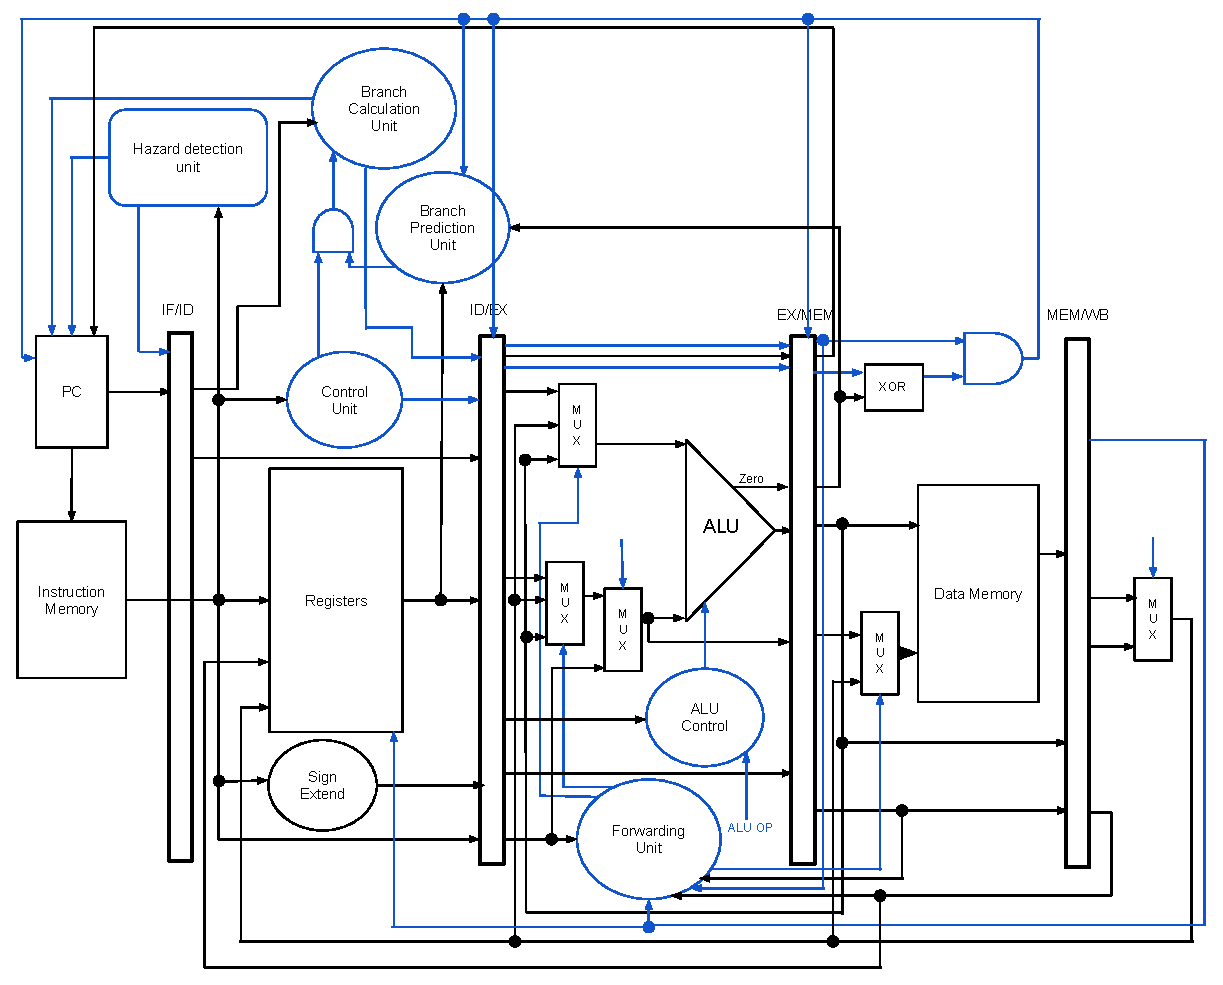
\includegraphics[width=\textwidth]{assets/RTL.pdf}
        \label{fig:architecture}
        \caption{Top view of architecture. Some parts, namely wires,
                 have been simplified to make the drawing clearer to understand.}
    \end{center}
\end{figure}

The design of the processor is based on the architecture provided in Figure 5.1 \cite[p. 50]{compendium}.
Major changes from a multi-cycle architecture include pipeline barriers\todo{Explain which pipeline barriers have been addded} to separate stages,
and a new combinatorial control unit (a state machine will not suffice as multiple instructions are executing at the same time).
The suggested architecture has been extended to support jumps, data forwarding, hazard detection, speculative execution and dynamic branch prediction.

\section{Implementation}

\subsection{Data Forwarding}
Often, instructions are dependent on data calculated in the instructions directly before it.
In a pipelined processor, values will sometimes not have been written back to a register at the time they are needed as operands in another instruction.
The simple solution to this problem would be to stall the processor for 1-2 cycles so that data is available when it is needed.
This is not an ideal solution, however, as it will render big parts of the pipelined unused at many times.
To solve this a dedicated data forwarding unit is implemented.

The data forwarding unit compares destination registers from the MEM and WB stages, with source registers in the EX stage.
If the registers that the EX stage reads has been written to in the last two cycles, the new value hasn't been stored yet.
The forwarding unit hotlinks the values straight into the ALU unit, which in turns skips the wait for the values to be written to memory.
We add a mux in front of both operands to the ALU in the EX stage, with signals from the data in the MEM and WB stages.
Control signals from the forwarding unit switch between regular input data read from the register file, data from the MEM stage and data from the WB stage.

In addition to forwarding from the MEM \& WB stages to the EX stage, we support forwarding from WB to the MEM stage.
This enables fast memory copies by executing a SW instruction the cycle directly following a LW.

\subsection {Hazard Detection}
The implemented data forwarding will not be able to handle all kinds of data hazards.
Specifically, an R-type instruction directly following a load instruction, where the load's destination register is one of the source registers of the R-type instruction, can not benefit from data forwarding.
This is because while the R-type instruction is in the execute stage, the load instruction is still only in the MEM stage, and the data will not be ready before the next cycle.

To work around this issue, a hazard detection unit will detect a load followed by a data-dependent instruction (this does not apply to store instructions, as data forwarding takes care of this case).
A stall flag is enabled when a load instruction is currently in its execute stage, while a dependent instruction is in the ID stage.
This causes the dependent instruction to remain in the ID stage for one extra cycle, while the load instruction progresses to the MEM stage.
To give the effect of a nop (an instruction that does not affect program execution) between them, the control signals for the dependent instruction are set to zero for one cycle.
At the same time, the PC needs to stall for one cycle, so no instructions are skipped.
The next clock cycle, the instruction enters the execute stage.
Then, data will be loaded from memory, and as it enters the WB stage, be forwarded to the EX stage.

\subsection{Branching}

This processor implements multiple branch-related improvements compared to a naive pipelined datapath.
These improvements allow for speculative execution of instructions, keeping the pipeline full at all times.

The improvements include:
\begin{enumerate}
  \item
    Moving branch decisions from the memory stage to the instruction decode stage, comparing register values in a dedicated equality unit.
    This allows for instant branches with no lost cycles when data hazards are absent.
  \item
    When operands are unavailable in the decode stage, one cannot decide whether to take the branch.
    By making an educated guess using a branch prediction unit the processor can speculatively execute instructions, keeping the pipeline filled.
  \item
    If a branch is taken wrongly (as confirmed by calculating the correct branching decision in the execute stage, correcting in the memory stage) only two pipeline stages have to be flushed.

    This turns branching from a required two cycles of pipeline bubbles (delayed branching) to a best case of zero downtime, and a worst case of two cycles flushed.
\end{enumerate}

To allow for zero-downtime branching, the program counter allows for instant updates, implemented via an internal bypass straight through to the instruction memory.
This allows us to update the PC to the target branch address the same cycle we decide to branch, thereby having the branch-target instruction ready at the next clock cycle.

Moving the branching decision to the decode stage requires us to make a branching choice even when branch operands aren't available.
This architecture implements speculation with the help of a globally shared saturating counter (informally known as a two bit predictor).
The saturating counter is a simple state machine with four states: Strongly not taken, Weakly not taken, Weakly taken, and Strongly Taken.
The prediction given is based on the current state, and whenever a branching decision is confirmed, the state is shifted towards that choice.

To confirm branch decisions, whether a branch was taken, the branch control signal and the pc of the branch not taken are passed down the pipeline to the memory stage.
In the memory stage, if the branch control signal turns out to be high and the branch taken and alu zero flag differ, the branch was wrongly taken.
Pipeline stages ID and EX will be flushed, and the program counter set to the pc value of the branch destination not taken.
